\documentclass[11pt]{article}
\usepackage[utf8]{inputenc}
\usepackage[T1]{fontenc}
\usepackage{minted}
\usepackage{graphicx}
\usepackage{hyperref}
\usepackage{CJKutf8}

\author{Student: Sean Wang, szw87 \\ Professor: Mohit Tiwari, Antonio Espinoza \\ Department of Electrical \& Computer Engineering \\ The University of Texas at Austin}
\date{\today}
\title{EE379K Enterprise Network Security Lab 1 Report}
\hypersetup{
 pdfauthor={Student: Sean Wang, szw87 \\ Professor: Mohit Tiwari, Antonio Espinoza \\ Department of Electrical \& Computer Engineering \\ The University of Texas at Austin},
 pdftitle={EE379K Enterprise Network Security Lab 1 Report},
 pdfkeywords={},
 pdfsubject={},
 pdfcreator={},
 pdflang={English}}

\begin{document}

\maketitle
\section*{Part 1 - Networking and Denial of Service}
\subsection*{Step 1 - Client and Server in C}
For step 1, the client and server in C were implemented to closely match the Python versions.
For simplicity, the client sends the same hard coded message each time, similar to the Python
client. The C client and server were tested with the Python client and server to ensure
cross-functionality and that the client implementation in both languages worked almost
identically. The only difference between the C client and Python client was the output of the
Python client showing
\begin{verbatim}
  From Server: b'INPUT LOWERCASE SENTENCE:'
\end{verbatim}
and the C client showing
\begin{verbatim}
  From Server: INPUT LOWERCASE SENTENCE:
\end{verbatim}
To build the server, compile it with:
\begin{minted}{bash}
  $ gcc -o server server.c
\end{minted}
Similarly for the client, compile it with:
\begin{minted}{bash}
  $ gcc -o client client.c
\end{minted}
To run them, simply execute either:
\begin{minted}{bash}
  $ ./server
  $ ./client
\end{minted}
\subsection*{Step 2 - DOS Attack}
For step 2, the DOS attack was implemented using a command line tool called \verb|hping3|~\cite{hping3}
using the options
\begin{minted}{bash}
  $ sudo hping3
      --count 15000 \           # number of packets
      --destport 12000 \        # destination port
      --rand-source \           # randomize source IP
      --flood \                 # send as fast as possible
      --syn \                   # send SYN packets
      127.0.0.2                 # destination IP
\end{minted}

These flags specify to stop sending packets to \verb|127.0.0.2:12000| after sending/receiving 15000
SYN packets, using randomized IP addresses to disguise the actual source and prevent the
server's SYN-ACK packets from reaching the actual source. Additionally, the \verb|--flood|
option just says to send packets as fast as possible.

As a result, the server receives many requests for establishing a connection, but because the
SYN-ACK sent from the server never reaches the actual sender of the initial SYN packet, the
3-way handshake is never completed and the server is left waiting on a response from what it
sees as many clients. This can be seen in Figure~\ref{fig:handshake}, with some packet details
cut out to ensure legibility.
\begin{figure}[htbp]
  \centering
  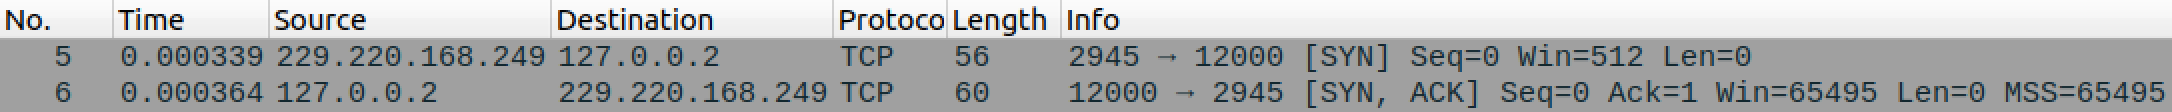
\includegraphics[width=1\linewidth]{./incomplete_handshake.png}
  \caption{\label{fig:handshake}
  An incomplete three-way handshake}
\end{figure}

Since the server is now swamped with connection requests, the real client (at IP \verb|127.0.0.1|)
cannot have its connection request processed by the server and times out, as shown in
Figure~\ref{fig:timeout}, also with some packet details cut out to ensure legibility.
\begin{figure}[htbp]
  \centering
  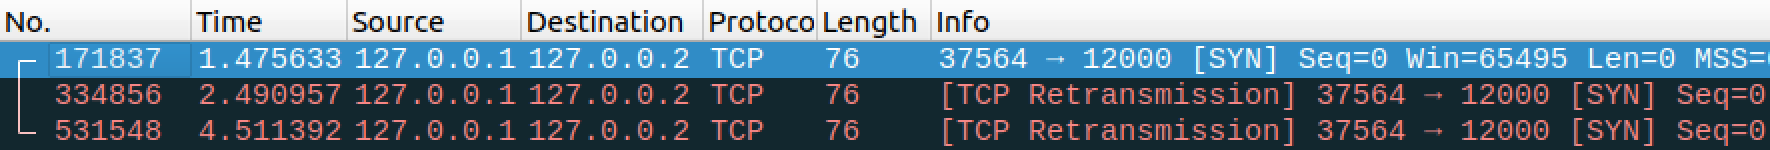
\includegraphics[width=1\linewidth]{./client_timeout.png}
  \caption{\label{fig:timeout}
  Client's sent SYN packet and client timeout}
\end{figure}

The rest of the tcpdump record of the DOS attack is in \verb|output.pcap| and shows the flood
of SYN packets sent to the server at IP \verb|127.0.0.2:12000|.
\section*{Part 2 - zmap scan}
For this part, a zmap scan~\cite{zmap} was run for about 2 hours and 47 minutes (10000 seconds) with the
following options:
\begin{minted}{bash}
  $ sudo zmap \
      --blacklist-file=blacklist.conf \ # subnets to exclude
      --target-port=80 \                # port number to scan
      --output-file=zmap_result.txt \   # output file
      --max-runtime=10000               # max runtime (seconds)
\end{minted}
The results of the zmap scan were:
\begin{verbatim}
  1261303 machines probed
  1534 machines responded
  0.12% hitrate
\end{verbatim}

Further information on each IP in the result list can be found using the \verb|whois| command, such
as the network the IP belongs in. This is specified by the Classless Inter-Domain Routing (CIDR)
info. In order to group all the IPs that belong in the same network, a Python and Bash script 
(\verb|network_whois.py| and \verb|whois_grep.sh|) were used to systematically run \verb|whois|
on each IP and capture the CIDR or inetnum to get the range of IPs that belong in the same network.
Then, using another Python script, \verb|analyze.py|, the IPs and other network information were
grouped accordingly into the following JSON files:
\begin{verbatim}
  - large_nets.json: list of networks that have multiple subnets
        (represented by multiple CIDRs)
  - net_ips.json: dictionary mapping a network's CIDR to a list
        of probed IPs in the network
  - net_sizes.json: dictionary mapping a network's CIDR to the
        number of probed IPs in the network
  - subnets.json: list of networks and their subnets
\end{verbatim}

Some notable observations were that there were some networks with a large range of IPs, so the 
\verb|whois| command would show several CIDRs to show the full span of the network. However,
sometimes the command would also return several fields of CIDRs, indicating that the probed IP
belonged to a subnetwork of a larger network, or even more nested than just two layers of
networks.

Digging deeper into a specific network, \verb|146.141.0.0/16|, it is owned by the African Network 
Information Center (AFRINIC), which is located in Ebene, Mauritius. This network is allocated 65,534
IPs, due to the '\verb|/16|' at the end of the CIDR, while only 6 machines responded when using
\verb|zmap| on port 80. Also, unlike some other networks, this network does not divide into any other
subnets. Using \verb|traceroute| on a specific IP that was probed in the initial \verb|zmap|,
\verb|146.141.234.183|, can show how many machines a packet must go through to reach the final
destination. In this case, it took 30 hops to reach \verb|146.141.234.183|. Additionally, running
\verb|zmap| on the network on port 22 gave almost 25,000 responses with a hitrate of 38.13\% in just
1000 seconds and running \verb|zmap| on the network on port 443 gave about 35,000 responses with a hitrate
of 53.72\% in just 1000 seconds. 
\section*{Part 3 - Internet Traffic On Different Connections}
For this part, a script (\verb|auto_collect.sh|) was used to automate accessing 10 different
websites 10 times each and recording network traffic with \verb|tcpdump|. This script was run
once per connection type (VPN, TOR, Firefox). Afterwards, another script (\verb|auto_summarize.sh|)
was used to automate summarizing the resulting \verb|.pcap| files for packets sent per access
and the average packet size per access. The collected data regarding the average number of packets
is summarized in Figure~\ref{fig:avg_packets} and the data regarding the average size of packets
is summarized in Figure~\ref{fig:avg_size}.

Using just a regular browser to access the websites, a passive device on the network can see
all kinds of information, including which websites were visited and the sizes of the packets. With a
VPN, \verb|tcpdump| captured information showing the client sending packets to the VPN server and
vice versa. However, information regarding packet source and destination were still visible. Finally,
using TOR, the captured network traffic showed mostly packets being sent to and from \verb|127.0.0.1|
and not the IP of, say, \verb|wikipedia.org|. As a result, it was much harder to tell exactly what
websites were visited just by looking at network traffic in Wireshark.

Although difficult, it is possible to determine which of the 10 websites was visited simply based on
connection statistics. For example, in Figure~\ref{fig:avg_size}, UC Berkeley's website has, on average,
larger packet sizes than most of the other websites, so given only these basic connection statistics,
guessing UC Berkeley's website as the site visited due to large packet sizes is not unreasonable.
Additionally, connection statistics that show a consistent rate packets sent and a consistent packet
size would most likely imply that a video or stream was being watched.

Some other observations of note were in regards to the number of packets sent per connection. The 
average number of packets sent each iteration of visiting the same website generally decreased as the
website was visited more. Also, since the websites were visited in a consistent order (from left to 
right on Figure~\ref{fig:avg_packets} and Figure~\ref{fig:avg_size}), there seemed to be a consistent
trend of decreasing average number of packets per connection. 
\begin{figure}[htbp]
  \centering
  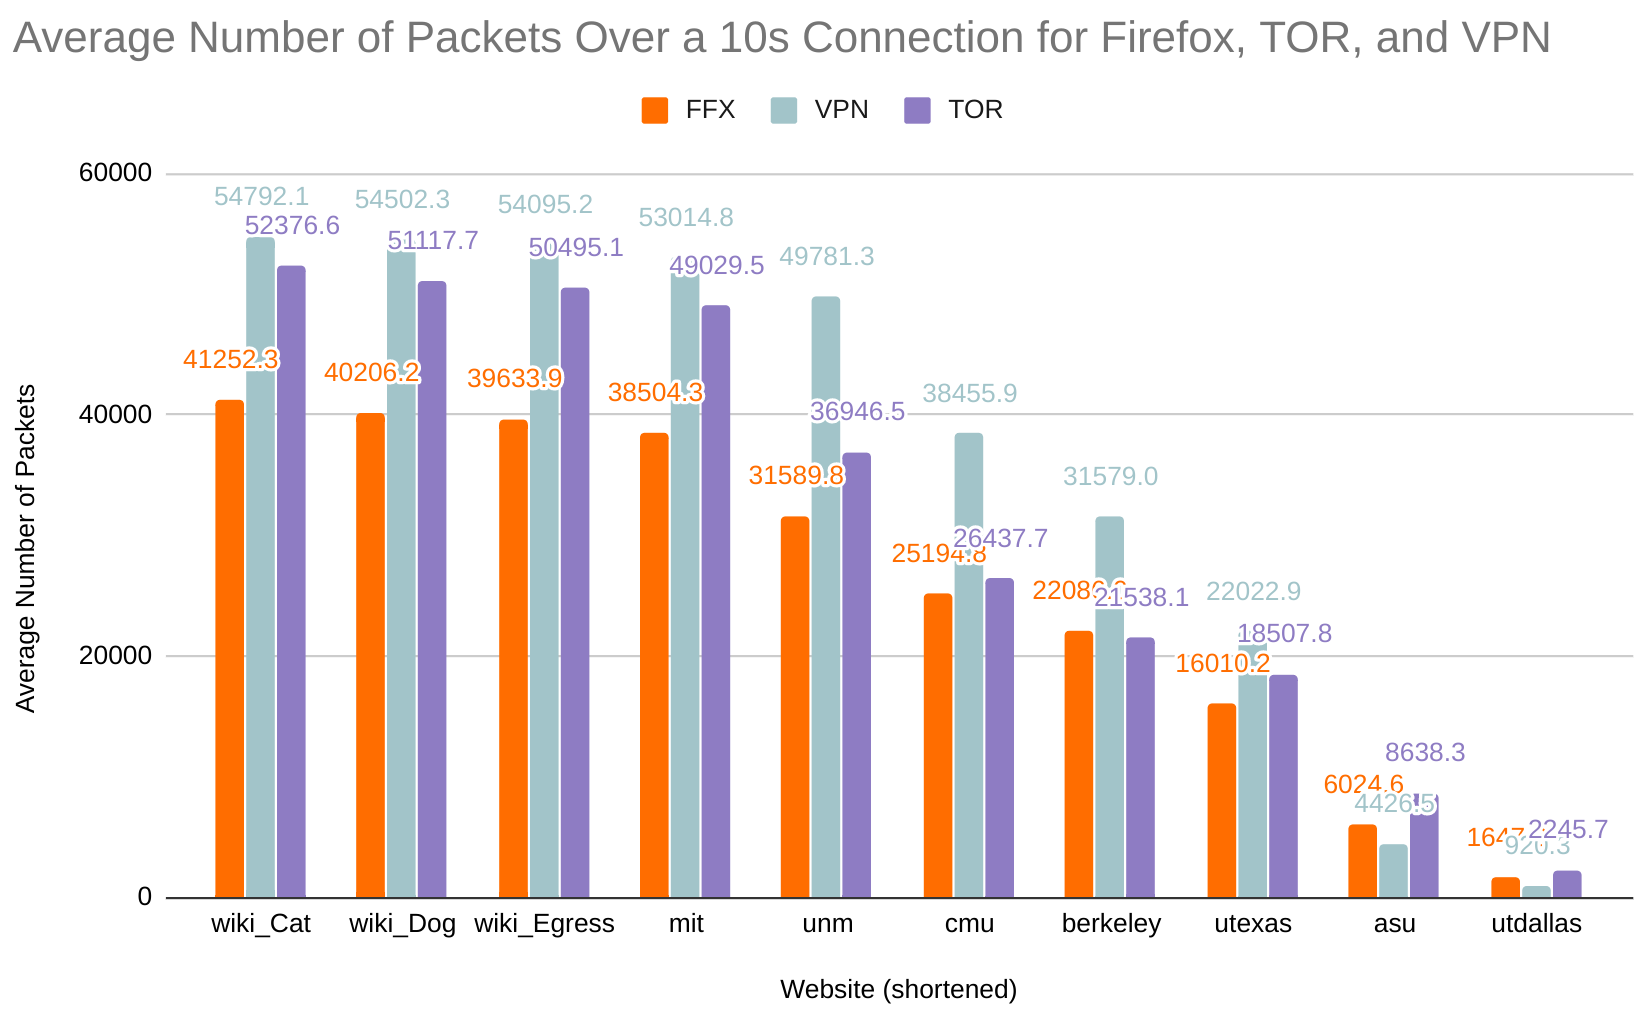
\includegraphics[width=.82\linewidth]{./average_packets.png}
  \caption{\label{fig:avg_packets}
  The average number of packets sent over a 10 second connection for 10 different websites on 3 different connections}
\end{figure}
\begin{figure}[!hbtp]
  \centering
  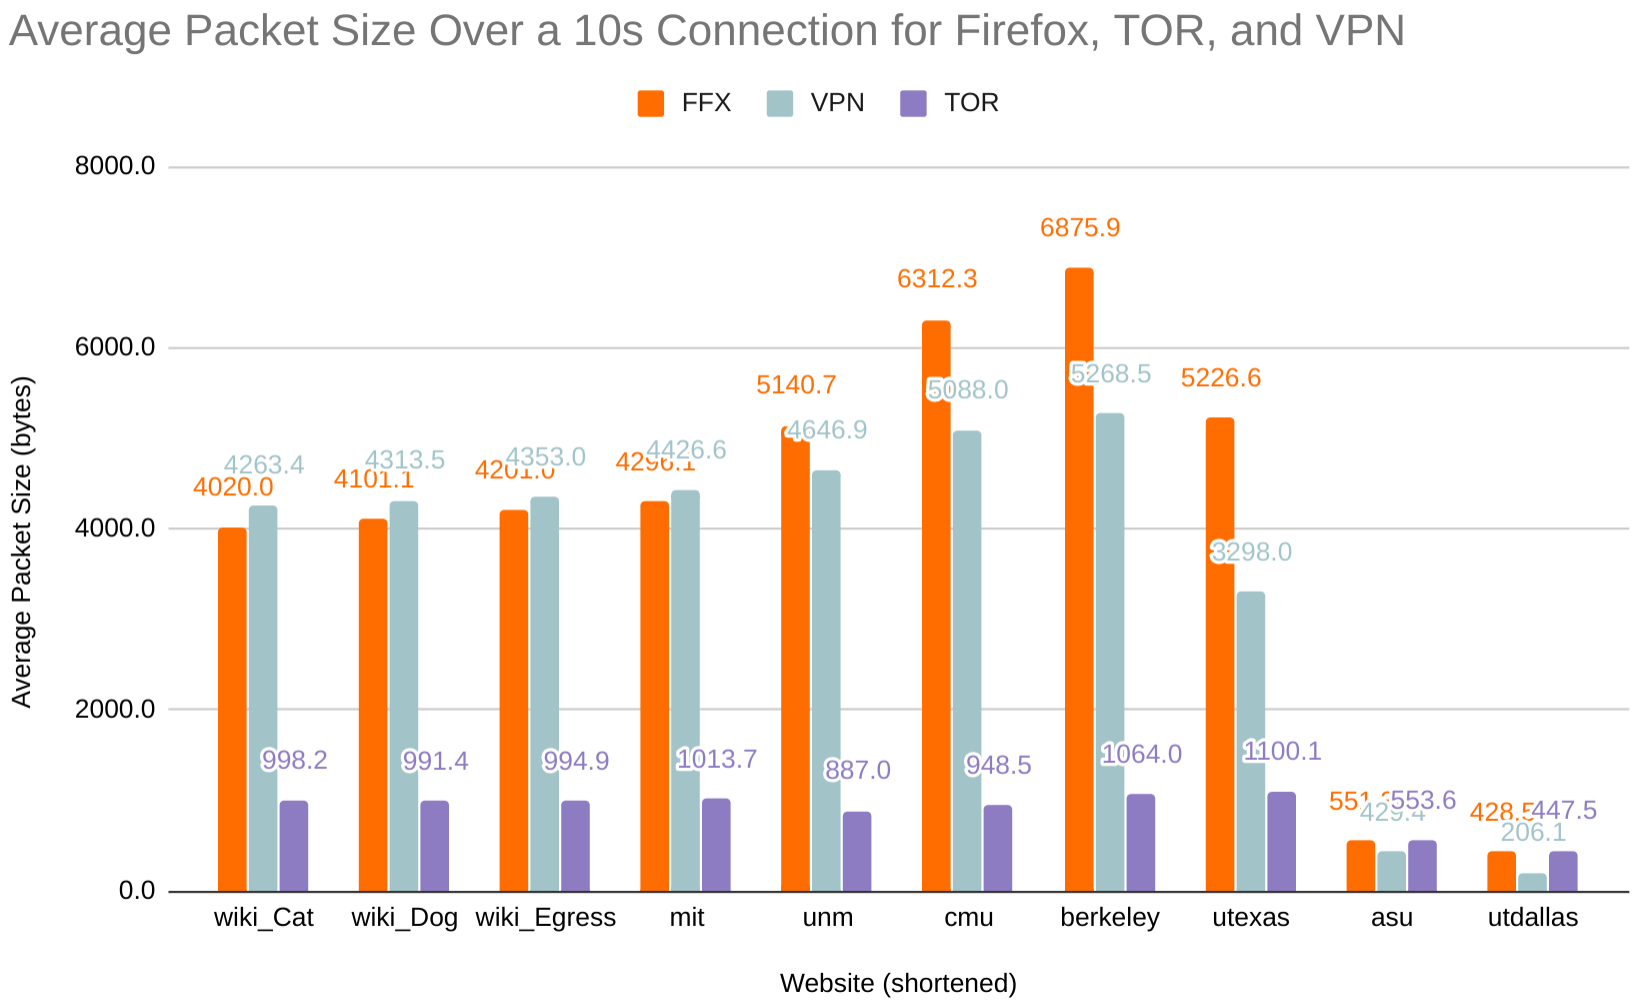
\includegraphics[width=.82\linewidth]{./average_size.png}
  \caption{\label{fig:avg_size}
  The average size of packets sent over a 10 second connection for 10 different websites on 3 different connections}
\end{figure}
\section*{Part 4 - Splitting Packets}
Using \verb|tcpdump| to record network traffic and Wireshark to view the packets, it is possible to
see certain details of a connection. In this part, these tools were used to analyze a connection to
http://baiwanzhan.com. Performing a generic search on the website resulted in an HTTP GET request
visible among the packets. Searching the phrase '\begin{CJK*}{UTF8}{gbsn}法轮\end{CJK*}' in the search
bar resulted in a connection reset. This is also visible in the \verb|.pcap| file as the client receiving
a reset TCP packet, seen as \verb|[RST]| in Wireshark. One way to get around this censorship would be to
split the packet into 2 and send the request split up in order to bypass the relay node that is intercepting
traffic and sending resets to censor certain words or phrases. This way, when the split packets reach the
destination, the server will reassemble the packets and view the result as one complete packet. This is
visible in Figure~\ref{fig:pkt_1} and Figure~\ref{fig:pkt_2}.
\begin{figure}[htbp]
  \centering
  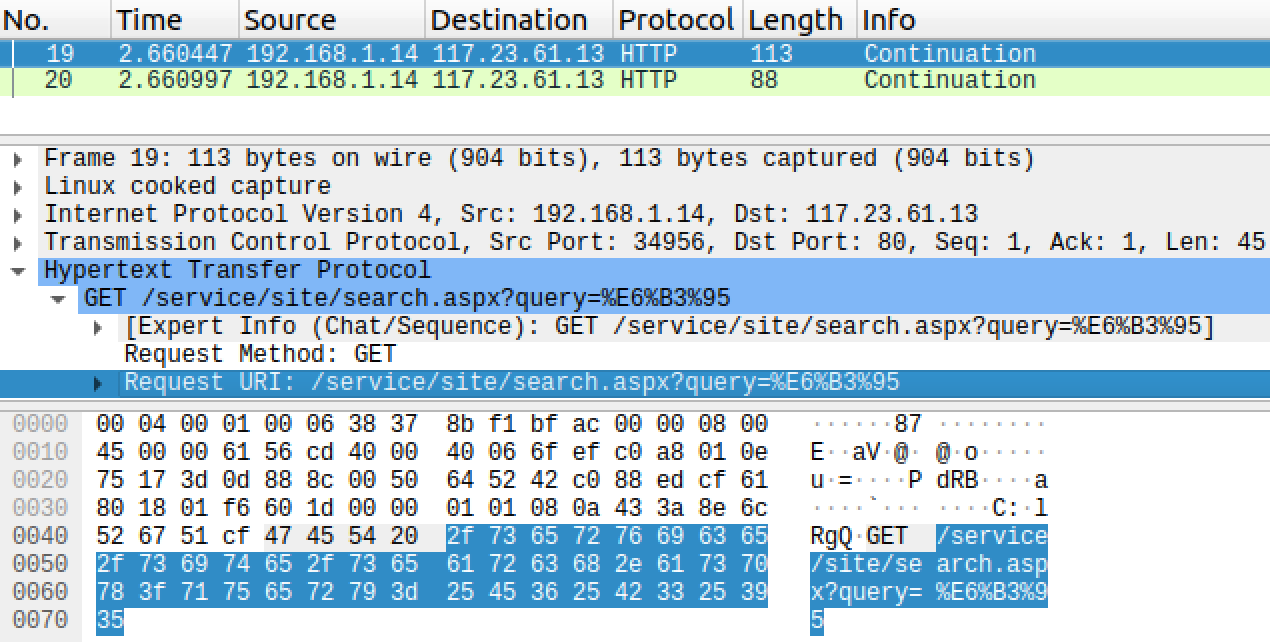
\includegraphics[width=.85\linewidth]{./packet1.png}
  \caption{\label{fig:pkt_1}
  The first half of the GET request. This includes the encoded first character.}
\end{figure}
\begin{figure}[htbp]
  \centering
  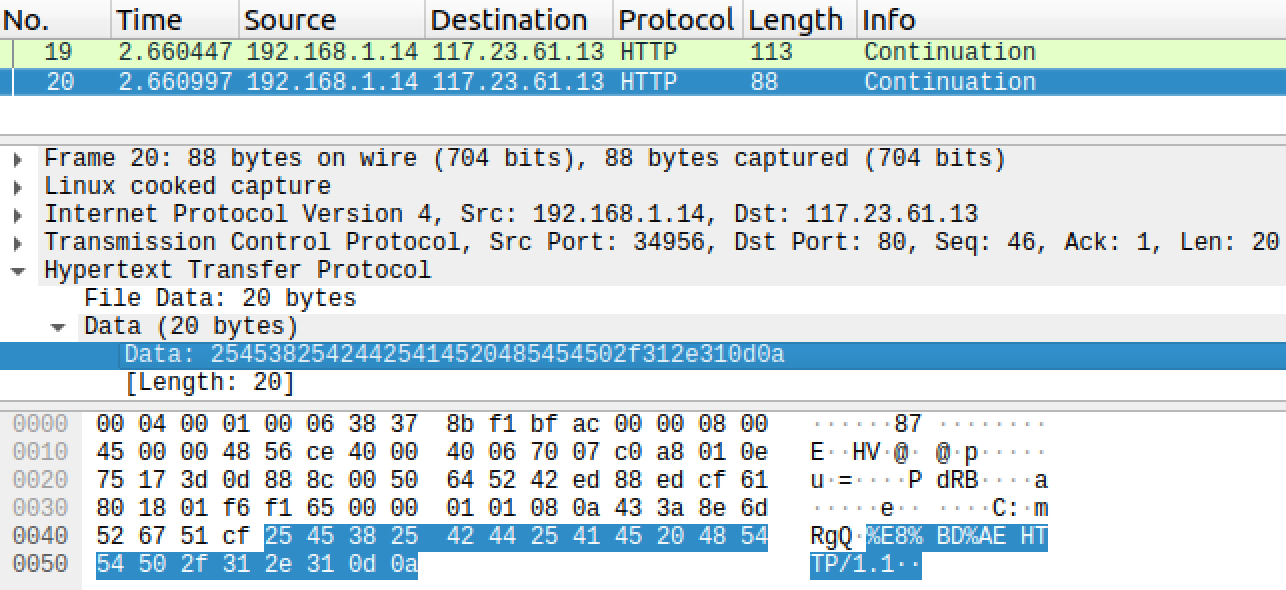
\includegraphics[width=.85\linewidth]{./packet2.png}
  \caption{\label{fig:pkt_2}
  The second half of the GET request. This includes the encoded second character.}
\end{figure}

However, the result of this was that the request still did not get through. This is certainly a possibility
since it would make sense for the censorship technology to be updated and close this loophole.

Using Wireshark to examine the packets from steps 2, where a generic search was performed, and from
step 3, where a search for the censored phrase was performed, it is revealed that the time to live (TTL)
of packets sent from the server is generally 43 seconds or 45 seconds. This is a relatively short TTL
and is probably in place to effectively balance traffic load and redirect traffic faster since the host
might be implementing a rerouting method where the IP on the authoritative DNS needs to be modified.
\section*{Conclusion}
Overall, this lab was very interesting, but was also a lot of work. It took around 35 hours since several
tasks that took a long time due to the nature of it (\verb|zmap| scan, accessing all the websites). 
Additionally, just figuring out how to process all the data from these tasks and what exactly to take note
of took a decent amount of time. Then, there was the task of writing the scripts to do data extraction
and analysis. The lab would be more enjoyable if there was less work, given that there is work from
other classes as well, but nonetheless, there was a lot to learn from each part of the lab, such as socket
programming in C, how a simple DOS attack works, and how to analyze network traffic in Wireshark.

\bibliography{bibliography}
\bibliographystyle{ieeetr}
\end{document}
